\documentclass[12pt,a4paper]{article}

\usepackage{polski} % Kodowanie znaków zostało wykonane w UTF-8 
\usepackage{indentfirst}
\usepackage{graphicx}
\usepackage{fancyhdr}
\usepackage{lastpage}
\usepackage{hyperref}
\usepackage{biblatex}
\usepackage{amsmath}

\title{Modelowanie epidemii}
\author{Krzysztof Kowalski}
\date{28 marca 2021}

\begin{document}
\maketitle
\thispagestyle{empty}
\newpage
\pagestyle{fancy}
\fancyhf{}
\rhead{Modelowanie epidemii}
\rfoot{Strona \thepage \hspace{1pt} z \pageref{LastPage}}
\tableofcontents
\newpage

\section{Cel dokumentu}
Niniejszy dokument zawiera informacje na temat sposobów modelowania epidemii. Opisuje on różne modele epidemiczne oraz sytuacje, w których powinno się je stosować. Dokument ten ma za zadanie przybliżyć temat modelowania epidemicznego oraz dać podstawy wiedzy potrzebnej do stworzenia projektu modelującego pandemię koronawirusa SARS-CoV-2, która rozpoczęła się pod koniec 2019 roku. 

\section{Modelowanie epidemii}
\subsection{Modelowanie deterministyczne}
Modelowanie deterministyczne polega na stworzeniu takiego modelu matematycznego opisującego pewny proces, w którym definiowanie stanów i przejścia między stanami są jednoznacznie określone za pomocą współczynników. Oznacza to, że w modelu takim nie ma losowości. Modele takie są opisywane równaniami różniczkowymi.

\subsection{Modelowanie stochastyczne}
Modelowanie stochastyczne jest podejście konkurencyjnym do modelowania deterministycznego. Polega ono na wykorzystaniu metod probabilistycznych do opisu przejść pomiędzy stanami. Tak więc w odróżnieniu od modelowania deterministycznego, w którym takie przejścia są reprezentowane za pomocą stałych współczynników, tutaj są one reprezentowane czystym prawdopodobieństwem. 

\subsection{Modele przedziałowe}
Modele przedziałowe polegają na tworzeniu modelu, w którym zbiór (np. społeczeństwo) jest dzielone na przedziały (np. stany zdrowia). Połączenia między przedziałami są definiowane za pomocą kierunku oraz stałego współczynnika z jakim zachodzi zmiana. 

\subsection{Model SIR}
Model SIR to jeden z najbardziej podstawowych modeli epidemiologicznych, który ma bardzo wiele modyfikacji. Składa się on z trzech klas. Na jego podstawie przedstawione zostanie co oznaczają poszczególne elementy w modelach i jak należy je interpretować. Dla bardziej rozbudowanych modeli tego typu logika ich tworzenia i interpretowania jest zbliżona, jednak liczba klas i parametrów je łączących się powiększa. 

Schemat modelu:
\begin{figure}[h!]
\centering
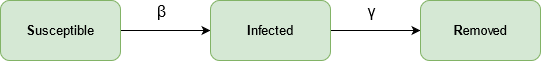
\includegraphics[width=1.0\textwidth]{Schematy/SIR}
\caption{Model SIR} 
\label{fig:Model SIR}
\end{figure}\\
\textit{S (Susceptible)} - osobniki podatne na zarażenie;\\
\textit{I (Infected)} - osobniki zarażone i zarażające innych;\\
\textit{R (Removed)} - osobniki wyzdrowiałe lub umarłe;\\
\textit{$\beta$} - współczynnik przenoszenia wirusa - częstość z jaką następuje zarażenie;\\
\textit{$\gamma$} - współczynnik pozbycia się wirusa - $\gamma = 1/D$, gdzie \textit{D} to średni czas trwania zaraźliwości;\\
\textit{N} - liczba wszystkich osobników w całej populacji.\\
Powyższy model można zapisać w postaci następującego układu równań różniczkowych:\\
$\dfrac{dS}{dt} = -\beta\cdot{S}\cdot\dfrac{I}{N}$\\
$\dfrac{dI}{dt} = \beta\cdot{S}\cdot\dfrac{I}{N} - \gamma\cdot{I}$\\
$\dfrac{dR}{dt} = \gamma\cdot{I}$\\
Poza tym należy zauważyć, że:
$\dfrac{dS}{dt} + \dfrac{dI}{dt} + \dfrac{dR}{dt} = 0$ oraz $S(t) + I(t) + R(t) = N$\\
Z powyższych równań po odpowiednich przekształceniach można oszacować współczynnik reprodukcji wirusa:
$ R_0  = \dfrac{\beta}{\gamma}$\\\\
Powyższe równania spełniają następujące założenia:
\begin{itemize}
\item Przyrost grupy osobników zainfekowanych jest proporcjonalny do liczby osobników podatnych oraz zainfekowanych - $\beta\cdot{S}\cdot{I}$;
\item Przyrost grupy osobników ozdrowiałych (usuniętych) jest wprost proporcjonalny do liczby osobników aktualnie chorych - $\gamma\cdot{I}$;
\item Brak okresu inkubacji, więc osobnik podatny, który się zaraził zaczyna chorować natychmiast;
\item Populacja jest dokładnie wymieszana, więc każdy typ osobnika ma jednakowe prawdopodobieństwo spotkania osobnika innego typu.
\end{itemize}

Są to jednak założenia opisane relatywnie ogólnie. Dlatego też powstało wiele modyfikacji modelu SIR, które dokładniej i wierniej odzwierciedlają pojedyncze choroby i infekcje. 

\subsection{Model SIR z dynamiką życiową}
Podstawowy model SIR nie uwzględnia dynamiki związanej z rodzeniem się nowych osobników oraz z umieraniem ich z przyczyn naturalnych. Taki model jest bardziej dokładny dla infekcji, które sa analizowane przez dłuższy okres czasu (np. lata). Dlatego można zmodyfikować go o dwa nowe współczynniki, które będą odpowiadać za rodzenie się nowych dzieci, które trafiają do klasy podatnej oraz za umieranie, które może się stać w każdej klasie:\\
\textit{$\Lambda$} - współczynnik urodzeń;\\
\textit{$\mu$} - współczynnik śmierci naturalnej.\\\\
Schemat modelu:
\begin{figure}[h!]
\centering
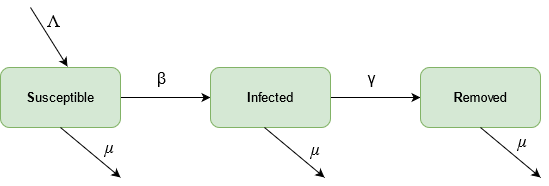
\includegraphics[width=1.0\textwidth]{Schematy/SIR_Vital}
\caption{Model SIR z dynamiką życiową} 
\label{fig:Model SIR z dynamiką życiową}
\end{figure}\\
Powyższy model można zapisać w postaci następującego układu równań różniczkowych:\\
$\dfrac{dS}{dt} = \Lambda - \mu\cdot{S} -\beta\cdot{S}\cdot\dfrac{I}{N}$\\
$\dfrac{dI}{dt} = \beta\cdot{S}\cdot\dfrac{I}{N} - \gamma\cdot{I} - \mu\cdot{I}$\\
$\dfrac{dR}{dt} = \gamma\cdot{I} - \mu\cdot{R}$\\

\newpage
\subsection{Model SIS}
Model SIS zakłada, że osobnik z grupy zarażającej (Infected) po wyzdrowieniu od razu trafia ponownie do grupy podatnej na zarażenie. Oznacza to, że przejście choroby nie daje żadnej odporności na daną chorobę i ponownie można na nią zachorować.\\
Schemat modelu:
\begin{figure}[h!]
\centering
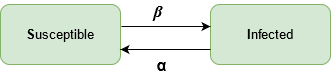
\includegraphics[width=0.5\textwidth]{Schematy/SIS}
\caption{Model SIS} 
\label{fig:Model SIS}
\end{figure}\\
\textit{$\alpha$} - współczynnik pozbycia się wirusa;\\\\
Powyższy model można zapisać w postaci następującego układu równań różniczkowych:\\
$\dfrac{dS}{dt} = -\beta\cdot{S}\cdot\dfrac{I}{N} + \alpha\cdot{I}$\\
$\dfrac{dI}{dt} = \beta\cdot{S}\cdot\dfrac{I}{N} - \alpha\cdot{I}$\\

\subsection{Model SIRS}
Model SIRS łączy cechy modelu SIR oraz SIS. Model ten zakłada, że osobnik po przebyciu choroby nabywa odporność na pewien czas, a następnie ponownie wraca do grupy podatnej na zakażenie.\\
Schemat modelu:
\begin{figure}[h!]
\centering
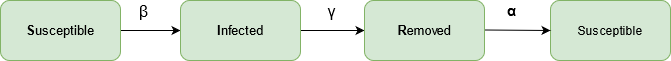
\includegraphics[width=1.0\textwidth]{Schematy/SIRS}
\caption{Model SIR} 
\label{fig:Model SIRS}
\end{figure}\\
Powyższy model można zapisać w postaci następującego układu równań różniczkowych:\\
$\dfrac{dS}{dt} =  \alpha\cdot{R} - \beta\cdot{S}\cdot\dfrac{I}{N}$\\
$\dfrac{dI}{dt} = \beta\cdot{S}\cdot\dfrac{I}{N} - \gamma\cdot{I}$\\
$\dfrac{dR}{dt} = \gamma\cdot{I} - \alpha\cdot{R}$

\subsection{Model SIRD}
Model SIRD różni się od modelu SIR tym, że występuje rozróżnienie między osobami, które po przebyciu infekcji wyzdrowiały oraz osobami, które umarły.\\
Schemat modelu:
\begin{figure}[h!]
\centering
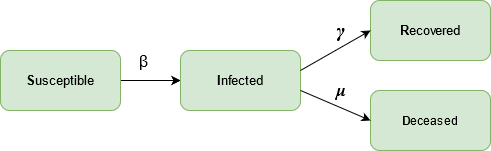
\includegraphics[width=1.0\textwidth]{Schematy/SIRD}
\caption{Model SIRD} 
\label{fig:Model SIRD}
\end{figure}\\
\textit{R (Recovered)} - osobniki, które wyzdrowiały po przebyciu infekcji;\\
\textit{D (Deceased)} - osobniki, które umarły po przebyciu infekcji;\\
Powyższy model można zapisać w postaci następującego układu równań różniczkowych:\\
$\dfrac{dS}{dt} = - \beta\cdot{S}\cdot\dfrac{I}{N-D}$\\
$\dfrac{dI}{dt} = \beta\cdot{S}\cdot\dfrac{I}{N-D} - \gamma\cdot{I} - \mu\cdot{I}$\\
$\dfrac{dR}{dt} = \gamma\cdot{I}$\\
$\dfrac{dD}{dt} = \mu\cdot{I}$


\subsection{Model SEIR}
Model SEIR stosowany jest w przypadkach, w których po zainfekowaniu występuje okres inkubacji. W tym czasie osobnik jest już zarażony, ale jeszcze nie zaraża innych osobników.\\
Schemat modelu:
\begin{figure}[h!]
\centering
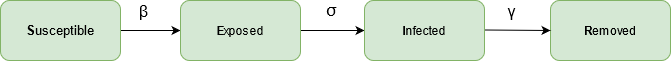
\includegraphics[width=1.0\textwidth]{Schematy/SEIR}
\caption{Model SEIR} 
\label{fig:Model SEIR}
\end{figure}\\
\textit{E (Exposed)} - osobniki, które uległy zarażeniu, ale nie zarażają;\\
\textit{ $\sigma$ } - współczynnik inkubacji - z jakim zarażeni stają się zarażającymi.\\
Powyższy model można zapisać w postaci następującego układu równań różniczkowych:\\
$\dfrac{dS}{dt} = - \beta\cdot{S}\cdot\dfrac{I}{N}$\\
$\dfrac{dE}{dt} = \beta\cdot{S}\cdot\dfrac{I}{N} - \sigma\cdot{E}$\\
$\dfrac{dI}{dt} = \sigma\cdot{E} - \gamma\cdot{I}$\\
$\dfrac{dR}{dt} = \gamma\cdot{I}$

\subsection{Model SEIQRD}
Model SEIQRD jest modelem, w którym występuje stała reprezentująca działania społeczności w celu zatrzymania rozprzestrzeniania się choroby. Jest to dodatkowa klasa zawierająca osobniki, które zostają objęte kwarantanną. Ponadto w tym modelu występuje rozróżnienie między śmiercią z powodu choroby i wyzdrowieniem. Model ten nie uwzględnia dynamiki życiowej (urodzenia i śmierć naturalna).\\
Schemat modelu:
\begin{figure}[h!]
\centering
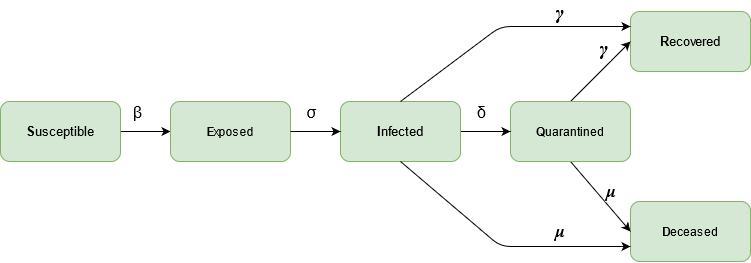
\includegraphics[width=1.0\textwidth]{Schematy/SEIQRD}
\caption{Model SEIQRD} 
\label{fig:Model SEIQRD}
\end{figure}\\
\textit{Q (Quarantined)} - osobniki, które po zarażeniu zostały objęte kwarantanną;\\
\textit{ $\delta$ } - współczynnik kwarantanny - częstość obejmowania kwarantanną osobników z grupy zarażonej.\\
$\dfrac{dS}{dt} = - \beta\cdot{S}\cdot\dfrac{I}{N-D-Q}$\\
$\dfrac{dE}{dt} = \beta\cdot{S}\cdot\dfrac{I}{N-D-Q} - \sigma\cdot{E}$\\
$\dfrac{dI}{dt} = \sigma\cdot{E} - \gamma\cdot{I} - \mu\cdot{I} - \delta\cdot{I}$\\
$\dfrac{dQ}{dt} = \gamma\cdot{I} - \mu\cdot{Q} - \gamma\cdot{Q}$\\
$\dfrac{dR}{dt} = \gamma\cdot{I} + \gamma\cdot{Q}$\\
$\dfrac{dD}{dt} = \mu\cdot{I} + \mu\cdot{Q}$

\subsection{Inne rozszerzone modele SEIR}
Poniższy model zakłada, że nie wszystkie przypadki zarażeń są zgłaszane i zapisywane. Może to być łagodnym przebiegiem choroby (lub bezobjawowym) lub niechęcią ludzi do zgłaszania się. Istnieją  zatem osobniki w grupie Unreported, którzy zarażają innych, lecz nie są sklasyfikowani jako osoby z wirusem. Jest w tym modelu stworzona również dodatkowa grupa na osoby hospitalizowane, które mają bardziej niebezpieczny przebieg choroby.  
Schemat modelu:
\begin{figure}[h!]
\centering
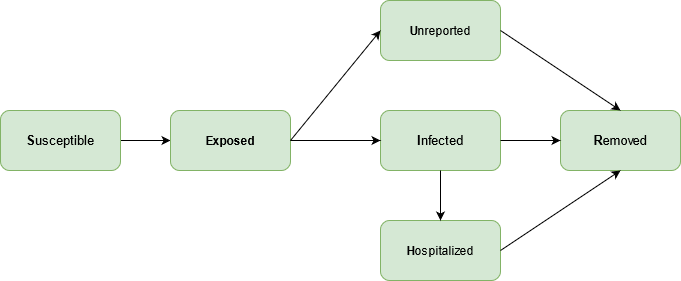
\includegraphics[width=1.0\textwidth]{Schematy/SEIR_ext_1}
\caption{Model SEIR rozszerzony} 
\label{fig:Model SEIR rozszerzony1}
\end{figure}


Kolejny model zakłada, że nie wszyscy ludzie z grupy zarażającej (Infected) są testowani. Ten model działa podobnie do poprzedniego modelu, ponieważ nie wszyscy ludzie zarażający są klasyfikowani jako ludzie z wirusem. Ponownie może to być związane z przechodzeniem choroby bezobjawowo. 
Schemat modelu:
\begin{figure}[h!]
\centering
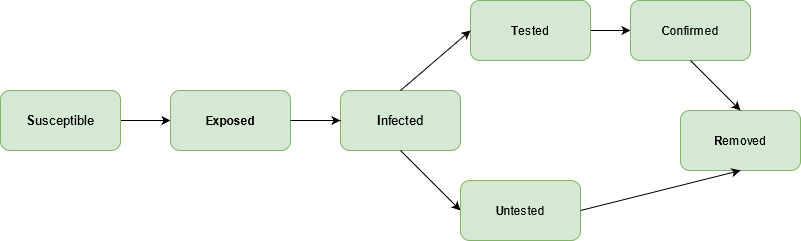
\includegraphics[width=1.0\textwidth]{Schematy/SEIR_ext_2}
\caption{Model SEIR rozszerzony} 
\label{fig:Model SEIR rozszerzony2}
\end{figure}



\end{document}